\documentclass[10pt]{article}

\usepackage[left=.5in, right=.5in, top=.3in, bottom=.5in]{geometry}
\usepackage{amsfonts,amsmath,amssymb}
\usepackage{authblk}
%% put affiliations into one line
\makeatletter
\renewcommand\AB@affilsepx{\quad\protect\Affilfont}
\usepackage{bbm}
\usepackage[inline]{enumitem}
\usepackage{graphicx}
\graphicspath{{./}{../image/}}
\usepackage[colorlinks=true,citecolor=blue,urlcolor=blue]{hyperref}
\usepackage{natbib}
\usepackage{setspace}
\setstretch{1.2}
\usepackage{titlesec}
\titlespacing*{\section}{0pt}{5pt}{5pt}

\newcommand{\EE}{{\mathbb{E}}}
\newcommand{\PP}{{\mathbb{P}}}
\newcommand{\QQ}{{\mathbb{Q}}}
\newcommand{\Fb}{\mathbf{F}}
\newcommand{\Ib}{\mathbf{I}}
\newcommand{\hb}{\mathbf{h}}
\newcommand{\xb}{\mathbf{x}}
\newcommand{\one}{\mathbbm{1}}
\newcommand{\Ocal}{\mathcal{O}}


\begin{document}


\title{\vspace{-1cm} \Large
Progress Report: Transformer-CRF Integration for Sequence Labeling on EEG Data}

\author[1]{Xiaohang Ma}
\author[2]{Shiying Xiao}
\author[2]{Xiaohui Yin}

\affil[1]{Department of Mathematics, UConn}
\affil[2]{Department of Statistics, UConn}

\date{\vspace{-1.3cm}}

\maketitle


\section{Progress}
% Overview of progress made and key accomplishments.


The project is progressing according to schedule. To date, we have made
significant strides in several key areas:
\begin{enumerate}
\item Model Development:
We have initiated development of a convolutional neural network (CNN) combined
with a hidden conditional random field (HCRF). This hybrid approach aims to
create a robust sequence labeling framework capable of capturing both local
and global dependencies within the data sequences.
\item Variational Inference Implementation:
To efficiently approximate the posterior distributions in our complex model,
we have integrated variational inference into the HCRF component.
This technique is particularly effective in handling the computational
challenges posed by the dataset's heterogeneity.
\item Data Visualization:
We have successfully visualized key features of the dataset.
\end{enumerate}
%This progress has provided a foundation for the next
%steps of our research.


\section{Preliminary Results}
% Summary of initial findings and analyses.


The potential of our HCRF model:
\begin{equation*}
\Phi(y, \hb, \xb; \theta) = \underbrace{
\sum_{j \in \nu} \phi(h_j, x_j; \omega) +
\sum_{i \neq j} \psi(h_i, h_j, x_i, x_j; \eta)}_{
% \propto \log\PP( \hb \vert \xb; \theta)
\textrm{Measures log-likelihood $\log\PP(\hb \vert \xb; \theta)$}}
+ \underbrace{
\sum_{j \in \nu} \varphi(y, h_j, x_j; \delta) + \vartheta(y, \xb; \varpi)
}_{
% \propto \log\PP(y | \hb, \xb; \theta)
\textrm{Measures log-likelihood $\log\PP(y \vert \hb, \xb; \theta)$}
}
\end{equation*}


\begin{itemize}
\item \textbf{Unary Potential}
$\phi(h_j, x_j; \omega)$ measures the likelihood of the local feature
$x_j$ is assigned as the hidden attention state $h_j$.
We generate the likelihood through a softmax operation on $\Fb(\xb)$
the feature maps of CNN with $(N, C_{\textrm{out}})$ dimensions,
by which the potential of each pixel $x_j$ assigned as each state of
hidden state set $\{0, 1, \dots, 5\}$
is drawn and represented by a matrix with $(N, 2)$ dimension.
\item The parameter $\omega$ is learned by our end-to-end CNN-Unet
training structure.
\item \textbf{Unary Potential} $\varphi(y, h_j; \delta)$ measures
the compatibility between global class label $y$ and the hidden local
state $h_j$. This potential is parametrized as:
\begin{align*}
\varphi(y, h_{j}; \delta) = \sum_{a \in Y} \sum_{b \in H} \delta_{a, b}
\cdot \one(y = a) \cdot \one(h_j = b).
\end{align*}
\item \textbf{Binary Potential} $\psi(h_i, h_j, x_i, x_j; \eta)$
balances the hidden label compatibility of the neighboring pixels on the 
feature image $\Fb(\Ib)$.
We define this potential through a common contrast-sensitive two-kernal 
potentials~\citep{krahenbuhl2011efficient,chen2022end}:
\begin{equation*}
\psi(h_i, h_j, x_i, x_j; \eta) = \mu(h_i, h_j) \Bigg[
\omega_1 \exp \left(
-\frac{\left\lvert p_i - p_j \right\rvert^2}{2\eta_\alpha^2}
-\frac{\left\lvert \Fb_i(\Ib) - \Fb_j(\Ib) \right\rvert^2}{2\eta_\beta^2} 
\right) + \omega_2 \exp \left(
- \frac{\left\lvert p_i - p_j \right\rvert^2}{2 \eta_\gamma^2}
\right)
\Bigg]
\end{equation*}
\end{itemize}


The mean-field varepsilon family approximation of
$\log\PP(\hb \vert y, \xb; \theta)$ as $\QQ(\hb) = \prod_{i=1}^N q_i(h_i)$.
Then the evidence lower bound under the mean-field family is given by
\begin{equation*}
\begin{split}
& \textrm{ELBO}(\QQ) = \EE_{\QQ(\hb)} \log\PP(y, \hb \vert \xb; \theta)
- \EE_{\QQ(\hb)} \log q(\hb) = \sum_{i=1}^N \EE_{q_i(h_i)}
\left[ \phi(h_j, x_j; \omega) + \varphi(y, h_j, x_j; \delta) \right]
+ \sum_{i=1}^N \sum_{j=1}^N \sum_{l,l^\prime} \one_{\{i \neq j\}}\QQ(h_i = l) \\
&\quad \QQ(h_j = l^\prime) \mu(l, l^\prime)
\Bigg[ \omega_1 \exp \left(
- \frac{\left\lvert p_i - p_j \right\rvert^2}{2\eta_\alpha^2}
- \frac{\left\lvert \Fb_i(\Ib) - \Fb_j(\Ib) \right\rvert^2}{2\eta_\beta^2}
\right)
+ \omega_2 \exp \left(
- \frac{\left\lvert p_i - p_j \right\rvert^2}{2\eta_\gamma^2}
\right) \Bigg]
- \sum_{i=1}^N \EE_{q_i} \log q_i(h_i) + \vartheta(y, \xb; \varpi).
\end{split}
\end{equation*}


By the coordinate ascent variational inference(CAVI) algorithm,
we can obtain that fix $q_j(h_j), \forall j \neq i$, the optimal $q_i(h_i)$
that maximizes $\textrm{ELBO}(q_i(h_i))$ is given by
$\QQ(h_i) \propto \exp\{\EE_{\QQ(\hb_{-i})}
\log\PP(y, h_i, \hb_{-i} \vert \xb; \theta)\}$.
Thus, we can get that


\begin{equation*}
q_i(l) = \frac{ \exp \left\{
\phi(h_j, x_j; \omega) + \varphi(y, h_j, x_j; \delta)
+ \sum_{j \neq i} \sum_{l^\prime} q(l^\prime) \mu(l, l^\prime) 
\left[ \omega_1 \exp \left(
- \frac{\left\lvert p_i - p_j \right\rvert^2}{2\eta_\alpha^2}
- \frac{\left\lvert \Fb_i(\Ib) - \Fb_j(\Ib) \right\rvert^2}{2\eta_\beta^2}
\right)
+ \omega_2 \exp \left(
- \frac{\left\lvert p_i - p_j 
\right\rvert^2}{2\eta_\gamma^2}
\right)
\right]
\right\}
}{Z_i}
\end{equation*}


While the models are still under development and optimization,
initial results are promising. For instance, Figure~\ref{fig:SEIZURE_3}
illustrates a sample prediction with ground truth 94.\% Seizure and 2.9\% LPD.
Our model predicts 88.4\% Seizure and 1.6\% LPD.
Yellow highlights indicate the regions where the model focused its attention.
These preliminary results show trends that are consistent with our initial
hypotheses. The visualizations have proven useful in pinpointing areas for
further investigation, and the derived formulas appear to be robust and
aligned with the expected model outcomes. Further analysis will refine
these findings and explore additional dimensions of data.


\begin{figure}[tbp]
\centering
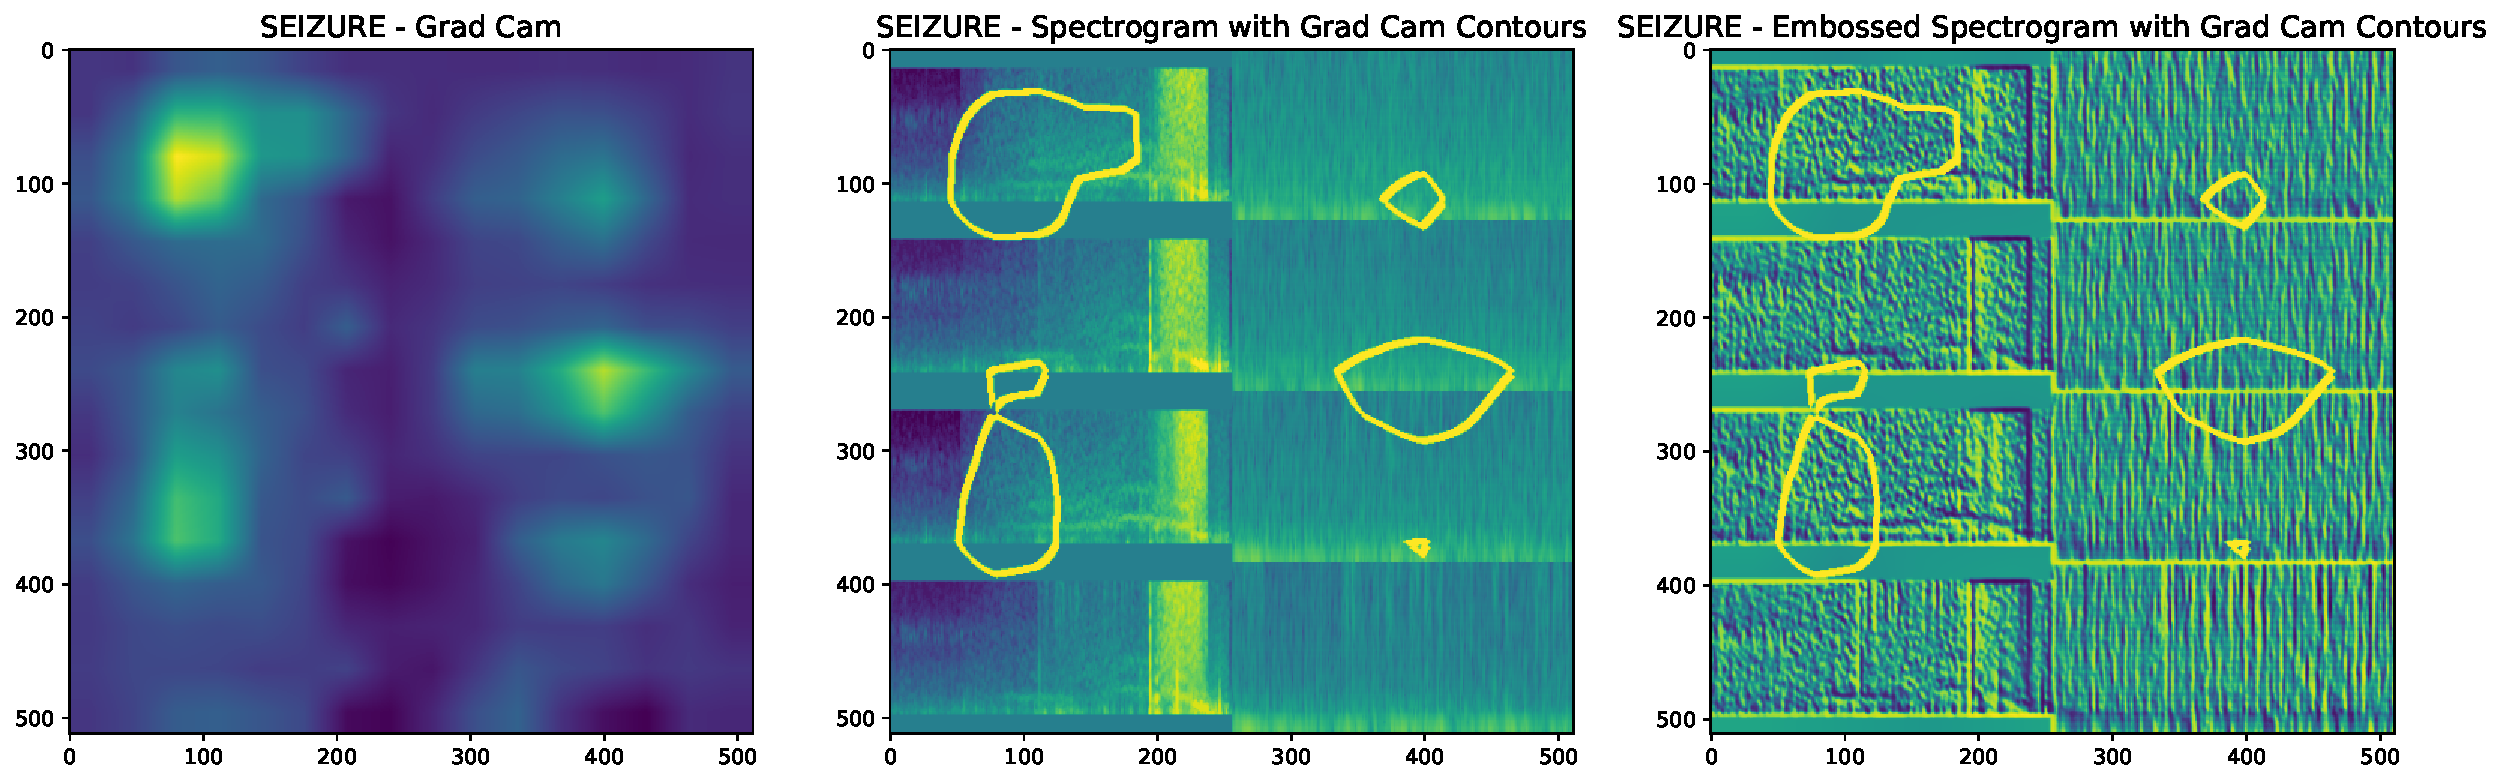
\includegraphics[width=.7\textwidth]{grad_cam_SEIZURE_3}
\caption{An example of data visualization. Areas highlighted in yellow
indicate regions where the model focused its attention during this specific
prediction.}
\label{fig:SEIZURE_3}
\end{figure}


\section{Challenges}
% Discussion of any challenges faced during the project.


We encountered minor challenges related to data handling and computational
limitations. In particular, the complexity of certain calculations required
additional processing time, which slightly delayed our progress.
We are currently exploring ways to optimize these computations.


\section{Plan Changes}
% Outline of any adjustments made to the original plan.


At this stage, we have not made significant changes to our original plan.
However, due to the complexity of the dataset and model, we may consider
slightly adjust the project timeline to allocate additional time for
model fine-tuning.


\section{Next Steps}
% Description of remaining tasks and strategy for completion.


The remaining tasks include:
\begin{enumerate*}[label = (\roman*)]
\item Expanding and refining the visualizations based on updated data.
\item Finalizing the derivation and validation of all essential formulas.
\item Conducting a comprehensive analysis with the refined model.
\item Preparing the final report and presentation materials.
\end{enumerate*}


\section{Updates}
% Additional relevant updates or future directions.


We will provide regular updates on model performance, challenges encountered,
and any significant changes to the project plan.


\bibliography{../manuscript/refs}
\bibliographystyle{chicago}

\end{document}

%%% Local Variables:
%%% mode: latex
%%% TeX-master: t
%%% End:
